\section{Sejarah Java}
\begin{figure}[!htbp]
    \centering
    
\includegraphics[scale=0.2]{pictures/104-1040733_kotlin-java-programming-language-logo-clipart-1024x598.png}
    \caption{Java}
    \label{}
\end{figure}
Java merupakan bahasa pemrograman yang dapat berjalan pada perangkat komputer maupun telepon genggam.  Bahasa ini dirilis pada tahun 1995 yang  dibuat oleh James Gosling  saat berada di Sun Microsystems  yang  saat ini merupakan bagian dari Oracle. bahasa pemrograman ini mengadopsi penulisan yang terdapat pada C dan C++ yang dikembangkan lagi menjadi sintaksis yang lebih sederhana.  Aplikasi  Dengan basis Java umumnya dikompilasi ke dalam bytecode Dan dapat dijalankan pada mesin virtual Java (JVM). Java  didesain  secara Khusus untuk memanfaatkan implementasi dependensi dengan sangat minimal. Dengan fungsionalitasnya  untuk  berjalan di beberapa platform  sistem operasi yang berbeda sehingga Java memiliki slogan Write once, run anywhere (WORA) atau bisa juga Write once, run everywhere (WORE). Java adalah bahasa pemrograman yang dapat digunakan untuk berbagai macam tujuan.  bahasa pemrograman concurrent, berbasis kelas, dan berorientasi objek. Bahasa ini dirancang secara khusus  untuk mengurangi ketergantungan ketika bahasa ini di terapkan. Hal ini yang dimaksudkan dalam slogannya "Write Once, Run Anywhere (WORA)". Slogan ini memiliki arti bahwa kode yang dijalankan pada suatu platform tidak perlu dikonfirmasi lagi pada platform lainnya. Java merupakan bahasa pemrograman yang paling populer digunakan dan dimanfaatkan dalam pengembangan berbagai jenis perangkat lunak aplikasi ataupun aplikasi lainnya.

Awalnya bahasa pemrograman ini diberi nama Oak, yang Merupakan nama sebuah pohon yang dapat dilihat oleh Gosling dari jendela kantornya. Kemudian dia memberi nama pemrograman ini dengan nama Green,  sehingga akhirnya dia mengganti namanya menjadi Java. Nama ini diambil dari kopi jawa yang banyak dikonsumsi oleh pencipta bahasa pemrograman ini. 

Ketika World Wide Web menjadi populer, Banyak kelebihan yang membuat bahasa ini dapat digunakan dengan baik dan cocok pada proyek maupun alat untuk adaptasi ke web. Pengembang bahasa ini merancang cara agar program berjalan aman pada halaman web dan hingga akhirnya dipilihlah nama yang baru untuk bahasa yaitu Java. Hingga sekarang Java menjadi bahasa pemrograman yang sangat populer digunakan. Aplikasi yang paling populer digunakan adalah aplikasi web client-server dengan 10 juta pengguna.

\section{Sejarah perkembangan}
Pada awalnya pemrograman Java berawal dari The Green Project yang berjalan untuk 18 bulan. Project ini dimulai pada 1991 hingga musim panas 1992. Proyek tersebut belum menggunakan versi Oak .  Proyek ini beranggotakan Patrick Naughton, Mike Sheridan, dan James Gosling, dan sembilan programmer lainnya dari Sun Microsystems.

Proyek ini berlangsung di gedung perkantoran di Sand Hill Road, Menlo Park. Pada saat musim panas 1992 proyek ini ditutup dengan menghasilkan sebuah program Java Oak yang ditujukan sebagai pengendali peralatan dengan teknologi touchscreen seperti sekarang. Teknologi ini diberi nama "*7" (Star Seven).

Setelah era Star Seven, perusahaan TV kabel tertarik untuk menambahkan beberapa orang dari proyek The Green Project. Mereka bekerja pada kantor di 100 Hamilton Avenue, Palo Alto. 

Dengan berjalannya waktu, perusahaan ini semakin maju. Jumlah karyawan yang meningkat dengan sangat signifikan dari 13 orang menjadi 17 orang. Pada saat itu, internet menjadi peran yang menjembatani ide di antara mereka. Pada awal tahun 1990, Internet belum terkenal seperti sekarang sehingga yang dipakai hanyalah untuk akademisi dan militer. Pada maret 1995, source code Java versi 1.0a2 dibuka. 

Ketika itu, pada pukul 04.00 di ruangan hotel Sheraton Pallace terjadi perpecahan di antara anggota proyek The Green Project. Tiga pimpinan proyek itu, Eric Schmidt, George Paolini, dan Masrc Andreessen dari Sun Microsystems membentuk perusahaan Netscape.

\section{Struktur Program}
Struktur program pada bahasa Java dibagi menjadi 4:
\begin{enumerate}
    \item Deklarasi Package\\
    Package merupakan sebuah folder yang diisi dengan  sekumpulan program Java. Deklarasi package biasanya dilakukan saat membuat aplikasi atau membuat program.\\
    Contoh deklarasi package:
    \begin{lstlisting}[language=Java]
package com.proyek.qeuangans;
    \end{lstlisting}
    Pada contoh diatas \textcolor{pred}{com.proyek} merupakan domain dari program proyek. Pada saat membuat program, kita boleh untuk tidak mendeklarasikan package, tetapi saat bagian produksi aplikasi kita wajib menuliskan package.

    \item Import Library\\
    Bagian ini melakukan import library yang dibutuhkan oleh program. Library adalah kumppulan dari class dan fungsi yang bisa kita gunakan ketika membuat program.\\
    Contoh Import Library:
    \begin{lstlisting}[language=Java]
import java.util.Scanner;
    \end{lstlisting}
    Pada contoh diatas, itu berarti kita mengimport class \textcolor{pred}{Scanner} dari sebuah package yang bernama \textcolor{pred}{java.util}

    \item Class\\
    Java merupakan bahasa pemrograman yang berbasis OOP (Object Oriented Programming) yang pada setiap program harus dibungkus di dalam class agar dapat dibuat menjadi objek. Class dibuka dengan kurung buka kurawal \{ dan kurung tutup kurawal \}. Dalam blok class dapat diisi dengan method, fungsi - fungsi dan variable.\\
    Contoh Class:
    \begin{lstlisting}[language=Java]
class NamaProgram {
    public static void main(String args[]){
        System.out.println("Halo Dunia!");
    }
}
    \end{lstlisting}
    Pada contoh program class tersebut terdapat method \textcolor{pred}{main()}. Method main ini akan di eksekusi pertama kali.

    \item Method Main\\
    Method main() merupakan blok program yang pertama kali dieksekusi. Method main() pada java wajib dibuat. Tanpa method main ini, maka program tidak bisa dieksekusi. Method main() memiliki parameter args[]. Parameter ini akan menyimpan sebuah nilai dari sebuah argumen di command line.\\
    Contoh method main:
    \begin{lstlisting}[language=Java]
public static void main(String args[]){
    System.out.println("Halo Dunia!");
}
    \end{lstlisting}

    Fungsi \textcolor{pred}{String args[]} pada baris program diatas adalah sebagai parameter yang berupa array yang memiliki tipe data srting. Parameter - parameter tersebut akan menampung argumen yang akan diberika ke program. 

\end{enumerate}

\subsection{Statement dan Ekspresi pada Java}
Statement dan ekspresi merupakan bagian yang terkecil dalam suatu program. Setiap statement dan ekspresi pada pemrograman java harus diakhiri dengan tanda titik koma (;). Statemen dan ekspresi akan menjadi instruksi yang akan dikerjakan oleh komputer.\\
Contoh Statement dan Ekspresi:
\begin{lstlisting}[language=Java]
System.out.println("Hello World");
System.out.println("Apa kabar?");
var x = 3;
var y = 8;
var z = x + y;
\end{lstlisting}

\subsection{Blok Program Java}
Blok program adalah kumpulan dari beberapa statement dan ekspresi yang dibungkus menjadi satu. Pada blok program ini harus selalu dibuka dengan kurung buka kurawal (\{) dan ditutup dengan kurung tutup kurawal (\}) Blok program dapat juga berisi blok program yang lain atau blok program didalam blok program.
\begin{lstlisting}[language=Java]
// blok program method main
public static void main(String args[]){
    System.out.println("Halo Dunia!");
    System.out.println("Halo para pembaca buku ini");

    // blok program percabangan if
    if( true ){
        System.out.println('True');
    }

    // blok program perulangan for 
    for ( int i = 0; i<10; i++){
        System.out.println("Perulangan ke"+i);
    }
}
\end{lstlisting}

\subsection{Penulisan Komentar pada Java}
Dalam sebuah program, akan ada bagian yang tidak akan pernah di sekssekusi ketika program dijalankan, bagian tersebut adalah komentar.\\
Penulisan komentar pada java sama seperti pada bahasa C. Java dapat mendefinisikan beberapa macam komentar yang diantaranya: 
\begin{itemize}
    \item Single-Line comment\\
    Single-Line comment merupakan penulisan komentar yang digunakan hanya untuk satu baris perintah saja. Biasanya komentar ini menggunakan garis miring ganda \textcolor{pred}{(//)}. Contoh penggunaan Single-Line comment: 
    \begin{lstlisting}[language=Java]
public static void main(String args[]){
    // ini adalah komentar satu baris
}
    \end{lstlisting}

    \item Multiline comment\\
    Multiline comment biasanya digunakan untuk banyak baris perintah atau beberapa baris perintah. Biasanya komentar ini menggunakan garis miring bintang \textcolor{pred}{(/*...*/)}. Contoh penggunaan Multiline comment:
    \begin{lstlisting}[language=Java]
public static void main(String args[]){
    /* awal penggunaan multiline comment
    for ( int i = 0; i<10; i++){
        System.out.println("Perulangan ke"+i);
    }
    akhir penggunaan multiline comment */

}
    \end{lstlisting}

    \item Documentation comment\\
    Documentation ini digunakan untuk menghasilkan file HTML dari program yang kit buat. Biasanya komentar ini dimulai dengan menggunakan tanda \textcolor{pred}{(/** ..... */)}. Contoh penggunaan Documentation comment:
    \begin{lstlisting}[language=Java]
/**
*
*
*
*@author D4TI2B (1184099 dan 1184094)
*@since 2020
*
*
*/
public static void main(String args[]){

}
    \end{lstlisting}

\end{itemize}
Komentar biasanya digunakan untuk beberapa hal:
\begin{enumerate}
    \item Memberi keterangan pada baris kode program
    \item Menonaktifkan fungsi atau method tertentu
    \item Membuat dokumentasi
    \item dll.
\end{enumerate}
%%%%%%%%%%%%%%%%%

\subsection{String dan Character}
String merupakan kumpulan dari Character. Biasanya kita mengetahuinya dengan nama teks. Contoh String:
\begin{lstlisting}[language=Java]
"Hello World"
\end{lstlisting}

Penulisan string pada Java wajib diapit oleh tanda petik ganda seperti pada contoh yang tertulis diatas. Jika diapit dengan tanda petik tunggual, maka dibuat menjadi character. Contoh penggunaan:
\begin{lstlisting}
'Hello world'
\end{lstlisting}

%Jadi harap dibedakan:
%\begin{enumerate}
%    \item Tanda petik ganda ("...") untuk membuat string;
%    \item Sedangkan tanda petik tunggal ('...') untuk membuat karakter.
%\end{enumerate}

\subsection{Case Sensitive}
Java memiliki sifat Case Sensitive, case sensitive disini berarti perbedaan huruf kapital dan huruf kecil harus diperhatikan karena banyak orang yang sering melakukan kesalahan dalam hal ini. Karena masih banyak orang yang belum bisa membedakan mana variabel yang menggunakan huruf besar dan huruf kecil.

\section{Mengenal Tipe Data Dasar di Java}
Tipe data merupakan bagian penting dalam pemrograman java. Tipe data biasanya akan digunakan dalam bentuk variabel variabbel. Java memiliki banyak tipe data dasar atau yang biasa dikenal tipe data primitif pada java. Tipe data dasar atau primitif dibagi menjadi empat bagian:
\begin{enumerate}
    \item Integer\\
    Integer merupakan tipe data untuk data bilangan bulat. Tipe data integer terbagi lagi menjadi empat bagian yaitu:
    \begin{itemize}
        \item byte
        \item short
        \item Int
        \item Long
    \end{itemize}
    Semakin besarnya tipe data maka akan semakin besar pula nilai yang dapat ditampung oleh tipe data tersebut.

    \item Floating Point\\
    Floating point merupakan type data rasional, tipe data ini dibagi menjadi dua bagian yaitu:
    \begin{itemize}
        \item Float
        \item Double 
    \end{itemize}

    \item Char\\
    Char merupakan simbol dari sebuah character. Terdapat kurang lebih 256 simbol yang terdaftar  dalam kode ASCII. 

    \medskip

    \noindent\fcolorbox{red}{yellow}{%
        \minipage[b]{\dimexpr\linewidth\fboxsep\fboxrule\relax}
        ASCII (American Standard Code for Information Interchange) merupakan Kode Standar Amerika untuk Pertukaran Informasi atau sebuah standar internasional dalam pengkodean huruf dan simbol secara universal. \cite{webmateridosen1}
        \endminipage}

    \medskip

    \item Boolean
    Boolean merupakan tipe data yang paling sederhana dalam pemrograman karena tipe data ini hanya memiliki dua jenis saja yaitu:
    \begin{itemize}
        \item True
        \item False
    \end{itemize}
    Nilai dari boolean ini, sering digunakan untuk mengatur alur dari jalannya program. Boolean lebih sering digunakan untuk percabangan pada program.
    \cite{ahmadi1}
    
\end{enumerate}

Berikut ini jangkauan nilai yang dapat diterapkan pada tipe data primitif diatas:
\begin{table}[htbp!]
    \begin{tabular}{|l|l|l|l|}
    \hline
    \rowcolor[HTML]{9AFF99} 
    \textbf{Tipe Data} & \textbf{Besar Storage} & \textbf{Nilai Minimal} & \textbf{Nilai Maksimal} \\ \hline
    Byte               & 8 bit (1 byte)         & -128                   & 127                     \\ \hline
    Short              & 16 bit (2 byte)        & -32768                 & 32767                   \\ \hline
    Int                & 32 bit (4 byte)        & -2147483648            & 2147483647              \\ \hline
    Long               & 64 bit (8 byte)        & -9223372036854775808   & 9223372036854775807     \\ \hline
    Float              & 32 bit (4 byte)        & 3.4 E-38              & 3.4 E+38               \\ \hline
    Double             & 64 bit (8 byte)        & 1.7 E-308             & 1.7 E+308              \\ \hline
    Char               & 16 bit (2 byte)        & \textbackslash{}uoooo  & \textbackslash{}uffff   \\ \hline
    \end{tabular}
    \caption{Jangkauan nilai tipe data primitif}
    \medskip
    \noindent\fcolorbox{red}{yellow}{%
        \minipage[h!]{\dimexpr\linewidth\fboxsep\fboxrule\relax}
        Tipe data tersebut dapat dibuat menjadi array. Tanda array adalah dengan adanya kurung siku "[]" pada saat setelah mengetik tipe data yang digunakan.
        \endminipage}
    \medskip
    \end{table}

\newpage
\section{Variabel}
Variabel adalah tempat untuk menampung sejumlah value pada memori. Jika dianalogikan, Variabel dapat dimisalkan seperti sebuah ruangan. 

Berikut ini adalah beberapa para ilmuan yang memberikan pengertian dari variabel :
\begin{enumerate}
    \item F.N Kerlinger\\
Pengertian variabel menurut F.N Kerlinger merupakan suatu konsep yang memiliki macam-macam nilai dari suatu konsep yang dapat di rubah. Sehingga konsep tersebut akan mendapatkan titik kesimpulan yang tepat dan terbaik. \cite{FNKerlinger}

    \item Sutrisno Hadi\\
Variabel merupakan variasi dari objek penelitian, seperti tinggi badan manusia yang divariasikan dengan berat badan maupun usia yang dimiliki. Sehingga menghasilkan nilai kuantitatif dari suatu penelitian yang diterapkan secara real atau nyata.

    \item Sugiono\\
Pengertian Variabel dari Sugiono merupakan segala sesuatu yang diproses melalui informasi tentang suatu hal dari penelitian untuk dipelajari dan mendapatkan hasil dari penelitian tersebut. Yang mana akan ada kesimpulan dari proses penelitiannya.

    \item Freddy Rankuti\\
Freddy Rankuti menerapkan variabel dengan artian suatu konsep yang memiliki nilai bervariasi. Yang mana nilai tersebut dibagi menjadi 4 data yang berbeda. Seperti rasio, skala, ordinal, nominal dan internal.

    \item Suharsimi Arikunto\\
Variabel merupakan objek penelitian yang menjadi perhatian pada suatu titik objek penelitian. Yang nantinya akan mendapatkan nilai dari kesimpulan suatu proses.

    \item Bagja Waluya\\
Konsep yang tidak pernah ketinggalan dalam setiap eksperimen yang dilakukan oleh seseorang. Dari eksperimen tersebut akan menghasilkan suatu data yang berguna sebagai bukti otentik suatu penelitian.

    \item Moh. Nazir\\
Berikutnya, mengenai pengertiaan variabel menurut Moh. Nazir adalah suatu konsep yang memiliki bermacam-macam nilai yang nyata. Dalam suatu penelitian yang menghasilkan garis besar dari adanya nilai kualitas dan kuantitas.

    \item Sugiarto\\
Menurut Sugiarto variabel adalah suatu karakter yang dapat di observasi dari unit amatan yang merupakan pengenal atau atribut dari anggota kelompok. Maksud dari variabel ini adalah terjadinya proses variasi antara objek satu dengan objek yang lain. Yang mana aturan masing-masing kelompok memiliki perbedaan variasi.

    \item Tri Mutiara\\
Suatu proses yang berjalan dengan baik hingga mendapat perhatian dengan fokus pada pengaruh nilai yang value. Itulah pengertian variabel menurut Tri Mutiara. Yang mengartikan variabel sebagai cara terbaik mendapatkan hasil penelitian.

    \item Bhisma Murti\\
Definisi variabel menurut bhisma murti adalah adanya fenomena yang memiliki variasi nilai pada sebuah observasi. Yang mana variasi nilai itu dapat di kukur dengan cara kualitatif dan kuantitatif. Sehingga menghasilkan data yang benar dan tepat.

    \item Dr Ahmad Watik Pratiknya\\
Konsep yang memiliki variabilitas dengan penggambaran suatu abstraksi dari fenomena tertentu. Yang mana konsep tersebut berupa data seperti asal kepemilikan ciri yang bervariasi, inilah yang disebut variabel.
\end{enumerate}

\textbf{Variabel pada java dibagi menjadi dua yaitu:}
\begin{itemize}
    \item Variabel Lokal\\
    Variabel lokal merupakan variabel yang hanya dapad diakses pada lingkup khusus saja. Variabel ini biasanya hanya bisa diakses pada prosedur atau fingsi dimana prosedur tersebut di deklarasikan. 
    \item Variabel Global\\
    Variabel Global merupakan variabel yang dapat diakses melalui semua lingkup dalam program yang dibuat. Variabel Global ini dapat digunakan oleh semua fungsi dan prosedur.
\end{itemize}

Untuk mendeklarasikan variabel, Kita harus menulis terlebih dahulu tipe data dari variabelnya, kemudian nama variabel, setelah itu kita wajib menginisiasi variabel tersebut agar tidak terjadi error. 

Berikut merupakan standar-standar dalam penulisan variabel:
\begin{enumerate}
\item Nama variabel biasanya diawali dengan huruf atau garis bawah. Contoh:
\begin{lstlisting}[language=Java]
nama = "Nama Kalian";
_nama = "Nama Kalian";
namaKu = "Nama Kalian";
nama_variabel = "Nama Kalian";
\end{lstlisting}

\item Karakter selanjutnya pada variabel dapat berupa huruf, garis bawah maupun angka. Contoh:
\begin{lstlisting}[language=Java]
__nama = "Nama Kalian"
nama1 = "Nama Kalian"
x1 = "Nama Kalian"    
\end{lstlisting}

\item  Nama variabel tidak boleh diawali dengan angka. Contoh:
\begin{lstlisting}[language=Java]
/* Penggunaan variabel ini salah karena diawali dengan angka */
3nama = "Nama Kalian"    
\end{lstlisting}

\item Penulisan variable bersifat Case-Sensitive (huruf besar dan huruf kecil sangant berpengaruh), contoh: 
\begin{lstlisting}[language=Java]
NAMA = "Nama Kalian"
nama = "Nama Kalian"
\end{lstlisting}
Variable nama dan NAMA pada contoh diatas merupakan variabel yang berbeda, dan memiliki arti yang berbeda.

\item Nama variabel yang digunakan tidak boleh menggunakan kata kunci yang ada pada bahasa pemrograman java (Reserved Word), contoh: 
\begin{lstlisting}[language=Java]
/* Penggunaan Variable seperti ini salah karena menggunakan reserved word pada java. */
if = "Nama saya: "
else = "Nama anda:"
while = "Nama kami:"    
\end{lstlisting}
\end{enumerate}


\section{Dasar - dasar Pemrograman}
\subsection{Operator}
Pada setiap pemrograman, operator merupakan peran penting karena tanpa adanya operator maka program tidak akan bisa berjalan dengan sempurna. Pada java, operator dibagi menjadi 6 jenis operator yaitu:
\begin{itemize}
    \item Operator Aritmatika
    \item Operator Penugasan
    \item Operator Logika
    \item Operator Pembanding 
    \item Operator Bitwise
    \item Operator Ternary
\end{itemize}

Dari keenam operator tersebut tentunya akan kami jabarkan satu per satu. 
\begin{enumerate}
    \item \textbf{Operator Aritmatika}\\
    Operator aritmatika digunakan untuk melakukan operasi aritmatika.
    \begin{table}[h!]
        \begin{center}
            \begin{tabular}{|l|l|}
                \hline
                \rowcolor[HTML]{9AFF99} 
                \textbf{Nama}           & \textbf{Simbol} \\ \hline
                Penjumlahan             & +               \\ \hline
                Pengurangan             & -               \\ \hline
                Perkalian               & *               \\ \hline
                Pembagian               & /               \\ \hline
                Sisa bagi (Mod/Modulus) & \%              \\ \hline
                \end{tabular}
        \end{center}      
        \caption{Operator Aritmatika}
    \end{table}

    Contoh penggunaan operator aritmatika pada program:
    \begin{lstlisting}[language=Java]
//Penjumlahan
total = angka1 + angka2;
System.out.println("Total = " + total);

//Pengurangan
total = angka1 - angka2;
System.out.println("Total = " + total);

//Perkalian
total = angka1 * angka2;
System.out.println("Total = " * total);

//Pembagian
total = angka1 / angka2;
System.out.println("Total = " + total);

//Modulus (sisa bagi)
total = angka1 % angka2;
System.out.println("Total = " + total);
    \end{lstlisting}

    \item \textbf{Operator Penugasan}\\
    Operator penugasan atau biasa disebut \textit{Assignment Operator} digunakan untuk memberikan sebuah tugas pada variable tertentu untuk mengisi nilai. Operator penugasan terdiri dari:
    \begin{table}[h!]
        \begin{center}
        \begin{tabular}{|l|l|}
            \hline
            \rowcolor[HTML]{9AFF99} 
            \textbf{Nama}             & \textbf{Simbol} \\ \hline
            Pengisian Nilai           & =               \\ \hline
            Pengisian dan Penambahan  & +=              \\ \hline
            Pengisian dan Pengurangan & -=              \\ \hline
            Pengisian dan Perkalian   & *=              \\ \hline
            Pengisian dan Pembagian   & /=              \\ \hline
            Pengisian dan Sisa bagi   & \%=             \\ \hline
            \end{tabular}
            \caption{Operator Penugasan}
        \end{center}
    \end{table}
    Contoh penggunaan operator penugasan:
    \begin{itemize}
        \item Pengisian Nilai
        \begin{lstlisting}[language=Java]
int x;
int y;

// Pengisian nilai
x = 5;
y = 10;
System.out.println("x : " + x);
System.out.println("y : " + y);
        \end{lstlisting}
        Hasil ketika program dijalankan:
        \begin{figure}[htbp!]
            \centering
            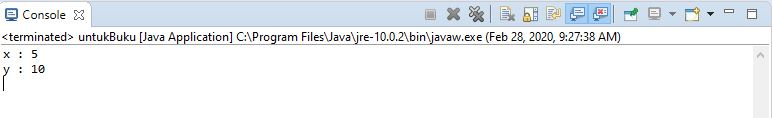
\includegraphics[scale=0.6]{pictures/Pengisian_Nilai_Operator_Penugasan.jpg}
            \caption{Hasil Pengisian Nilai Operator Penugasan}
            \label{}
        \end{figure}

        \item Penambahan
        \begin{lstlisting}[language=Java]
int x;
int y;
x = 5;
y = 10;

// penambahan
y += x;

// Hasil y menjadi 15
System.out.println("Penambahan : " + y);
        \end{lstlisting}
        Hasil ketika program dijalankan:
        \begin{figure}[htbp!]
            \centering
            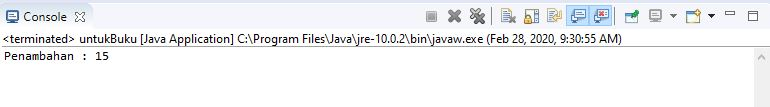
\includegraphics[scale=0.6]{pictures/penambahan_operator_penugasan.JPG}
            \caption{Hasil Penambahan Operator Penugasan}
            \label{}
        \end{figure}

        \item Pengurangan
        \begin{lstlisting}[language=Java]
int x;
int y;
x = 5;
y = 10;

// Pengurangan 
y -= x;

// Hasil y menjadi 5
System.out.println("Pengurangan : " + y);
        \end{lstlisting}
        Hasil ketika program dijalankan:
        \begin{figure}[htbp!]
            \centering
            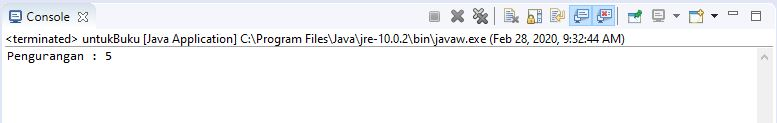
\includegraphics[scale=0.6]{pictures/pengurangan_operator_penugasan.JPG}
            \caption{Hasil Pengurangan Operator Penugasan}
            \label{}
        \end{figure}

        \item Perkalian
        \begin{lstlisting}[language=Java]
int x;
int y;
x = 5;
y = 10;

// Perkalian 
y *= x;

// Hasil y menjadi 50
System.out.println("Perkalian : " + y);
        \end{lstlisting}
        Hasil ketika program dijalankan:
        \begin{figure}[htbp!]
            \centering
            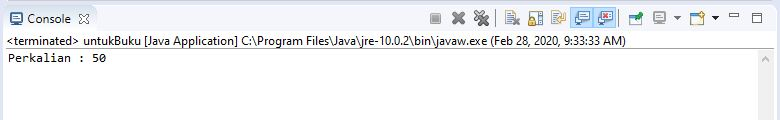
\includegraphics[scale=0.6]{pictures/perkalian_operator_penugasan.JPG}
            \caption{Hasil Perkalian Operator Penugasan}
            \label{}
        \end{figure}
\newline
        \item Pembagian
\begin{lstlisting}[language=Java]
int x;
int y;
x = 5;
y = 10;

// Pembagian 
y /= x;

// Hasil y menjadi 2
System.out.println("Pembagian : " + y);
\end{lstlisting}
\begin{figure}[htbp!]
    \centering
    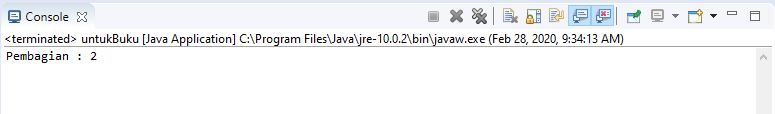
\includegraphics[scale=0.6]{pictures/pembagian_operator_penugasan.JPG}
    \caption{Hasil Pembagian Operator Penugasan}
    \label{}
\end{figure}

        \item Sisa bagi
        \begin{lstlisting}[language=Java]
int x;
int y;
x = 5;
y = 10;

// Pengurangan 
y %= x;

// Hasil y menjadi 0
System.out.println("Sisa Bagi : " + y);
        \end{lstlisting}
        Hasil ketika program dijalankan:
        \begin{figure}[htbp!]
            \centering
            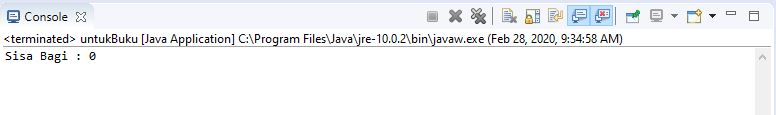
\includegraphics[scale=0.6]{pictures/sisa_bagi_operator_penugasan.JPG}
            \caption{Hasil Sisa Bagi Operator Penugasan}
            \label{}
        \end{figure}
    \end{itemize}

    \newpage
    \item \textbf{Operator Logika}\\
    Operator Logika merupakan operator yang akan sering kalian temui pada saat membuat sebuah program. Operator logika hanya bernilai \textbf{true} atau \textbf{false}. Jenis - jenis operator logika:
    \begin{table}[h!]
        \centering
        \begin{tabular}{|l|l|}
        \hline
        \rowcolor[HTML]{9AFF99} 
        \textbf{Nama}      & \textbf{Simbol} \\ \hline
        Logika AND         & \&\&            \\ \hline
        Logika OR          & ||              \\ \hline
        Negasi / Kebalikan & !               \\ \hline
        \end{tabular}
        \caption{Operator Logika}
    \end{table}

    Contoh penggunaan operator:
    \begin{itemize}
        \item \textbf{Logika AND}
        \begin{lstlisting}[language=Java]
public static void main(String[] args) {
    int a = 5;
    int b = 10;
    //Hasil Perbandingan a dan b benar keduanya maka Hasil = true
    boolean hasil_satu = (a > 1) && (b > 5);
    System.out.println("Hasil Pertama: " + hasil_satu);
    
    //Hasil Perbandingan a dan b hanya benar salah satunya saja maka Hasil = false
    boolean hasil_dua = (a > 1) && (b < 5);
    System.out.println("Hasil Kedua: " + hasil_dua);
}            
        \end{lstlisting}
        Hasil dari program tersebut adalah:
        \begin{figure}[htbp!]
            \centering
            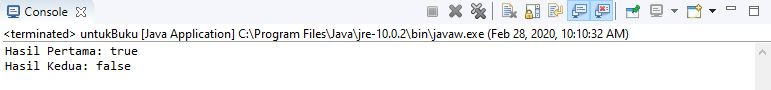
\includegraphics[scale=0.6]{pictures/hasil_operator_logika_AND.JPG}
            \caption{Hasil Operator Logika AND}
            \label{}
        \end{figure}

        \item \textbf{Logika OR}
        \begin{lstlisting}[language=Java]
public static void main(String[] args) {
    int a = 5;
    int b = 10;
                
    //Hasil Perbandingan a dan b hanya benar salah satunya, Tertapi jika menggunakan logika OR meskipun hanya benar salah satu maka akan menghasilkan nilai true
    boolean hasil_satu = (a > 1) || (b < 5);
    System.out.println("Hasil Kedua: " + hasil_satu);
}            
        \end{lstlisting}
        Hasil dari program tersebut adalah:
        \begin{figure}[htbp!]
            \centering
            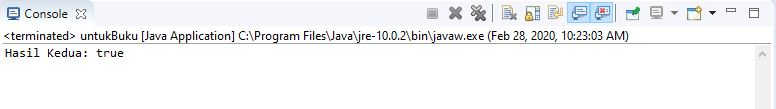
\includegraphics[scale=0.6]{pictures/hasil_operator_logika_OR.JPG}
            \caption{Hasil Operator Logika OR}
            \label{}
        \end{figure}

        \item \textbf{Negasi / Kebalikan}
        \begin{lstlisting}[language=Java]
public static void main(String[] args) {
    int a = 5;
    int b = 10;
                
    boolean hasil_dua = !((a < 15) ^ (b > 6));
    System.out.println("Hasil Kedua: " + hasil_dua);
}
        \end{lstlisting}
        Hasil dari program tersebut adalah:
        \begin{figure}[htbp!]
            \centering
            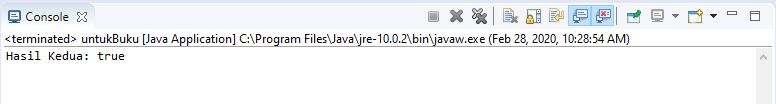
\includegraphics[scale=0.6]{pictures/hasil_operator_logika_negasi.JPG}
            \caption{Hasil negasi/kebalikan}
            \label{}
        \end{figure}

    \end{itemize}
    Pada penggunaan operator logika ini, kita dapat melihat tabel kebenaran untuk mendapatkan hasil dari logika.
    \begin{table}[h!]
        \centering
        \begin{tabular}{|l|l|c|c|}
            \hline
            \rowcolor[HTML]{9AFF99} 
            \textbf{Pernyataan 1}        & \textbf{Pernyataan 2}        & \multicolumn{1}{l|}{\cellcolor[HTML]{9AFF99}\textbf{AND}} & \multicolumn{1}{l|}{\cellcolor[HTML]{9AFF99}\textbf{OR}} \\ \hline
            {\color[HTML]{3166FF} true}  & {\color[HTML]{3166FF} true}  & {\color[HTML]{3166FF} true}                               & {\color[HTML]{3166FF} true}                              \\ \hline
            {\color[HTML]{3166FF} true}  & {\color[HTML]{FE0000} false} & {\color[HTML]{FE0000} false}                              & {\color[HTML]{3166FF} true}                              \\ \hline
            {\color[HTML]{FE0000} false} & {\color[HTML]{3166FF} true}  & {\color[HTML]{FE0000} false}                              & {\color[HTML]{3166FF} true}                              \\ \hline
            {\color[HTML]{FE0000} false} & {\color[HTML]{FE0000} false} & {\color[HTML]{FE0000} false}                              & {\color[HTML]{FE0000} false}                             \\ \hline
            \end{tabular}
        \caption{Tabel Kebenaran}
        \end{table}


\newpage
    \item \textbf{Operator Perbandingan}\\
    Operator perbandingan fungsinya adalah membandingkan. Operator ini akan menghasilkan nilai berupa boolean. Boolean berarti hasil ini hanya berupa \textbf{true} atau \textbf{false}. Jenis - jenis operator logika:
    \begin{table}[h!]
        \centering
        \begin{tabular}{|l|c|}
        \hline
        \rowcolor[HTML]{9AFF99} 
        \textbf{Nama}           & \multicolumn{1}{l|}{\cellcolor[HTML]{9AFF99}\textbf{Simbol}} \\ \hline
        Lebih Besar             & \textgreater{}                                               \\ \hline
        Lebih Kecil             & \textless{}                                                  \\ \hline
        Sama Dengan             & ==                                                           \\ \hline
        Tidak Sama Dengan       & !=                                                           \\ \hline
        Lebih Besar Sama Dengan & \textgreater{}=                                              \\ \hline
        Lebih Kecil Sama Dengan & \textless{}=                                                 \\ \hline
        \end{tabular}
        \caption{Operator Perbandingan}
        \end{table}

        Contoh penggunaan operator:
        \begin{itemize}
            \item \textbf{Lebih Besar}
            \begin{lstlisting}[language=Java]
public static void main(String[] args) {
    int A = 12;
    int B = 4;
    boolean hasil;
            
    // Apakah nilai A lebih besar dari nilai B?
    hasil = A > B;
    System.out.println(hasil);
}                
            \end{lstlisting}
            Hasil Eksekusi Program:
            \begin{figure}[htbp!]
                \centering
                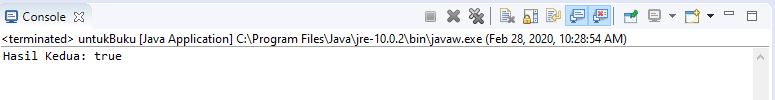
\includegraphics[scale=0.6]{pictures/operator_perbandingan_lebih_besar.JPG}
                \caption{Hasil operator lebih besar}
                \label{}
            \end{figure}
            \newpage
            \item \textbf{Lebih Kecil}
            \begin{lstlisting}[language=Java]
public static void main(String[] args) {
    int A = 12;
    int B = 4;
    boolean hasil;

    // Apakah nilai A lebih kecil dari nilai B?
    hasil = A < B;
    System.out.println(hasil);
}
            \end{lstlisting}
            Hasil Eksekusi Program:
            \begin{figure}[htbp!]
                \centering
                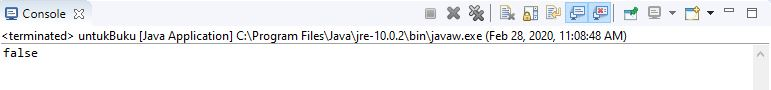
\includegraphics[scale=0.6]{pictures/operator_perbandingan_lebih_kecil.JPG}
                \caption{Hasil operator lebih kecil}
                \label{}
            \end{figure}

            \item \textbf{Sama Dengan}
            \begin{lstlisting}[language=Java]
public static void main(String[] args) {
    int A = 12;
    int B = 4;
    boolean hasil;

    // Apakah nilai A sama dengan nilai B?
    hasil = A == B;
    System.out.println(hasil);
}
            \end{lstlisting}
            Hasil Eksekusi Program:
            \begin{figure}[htbp!]
                \centering
                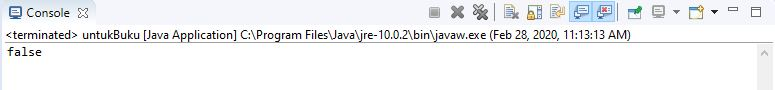
\includegraphics[scale=0.6]{pictures/operator_perbandingan_sama_dengan.JPG}
                \caption{Hasil operator sama dengan}
                \label{}
            \end{figure}

            \item \textbf{Tidak Sama Dengan}
            \begin{lstlisting}[language=Java]
public static void main(String[] args) {
    int A = 12;
    int B = 4;
    boolean hasil;
            
    // Apakah nilai A tidak sama dengan nilai B?
    hasil = A != B;
    System.out.println(hasil);
}
            \end{lstlisting}
            Hasil Eksekusi Program:
            \begin{figure}[htbp!]
                \centering
                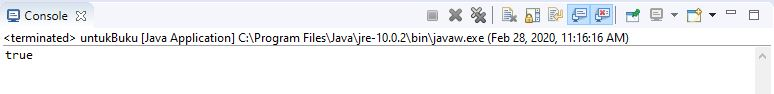
\includegraphics[scale=0.6]{pictures/operator_perbandingan_tidak_sama_dengan.JPG}
                \caption{Hasil operator tidak sama dengan}
                \label{}
            \end{figure}

            \item \textbf{Lebih Besar Sama Dengan}
            \begin{lstlisting}[language=Java]
public static void main(String[] args) {
    int A = 12;
    int B = 4;
    boolean hasil;
            
    // Apakah nilai A lebih besar atau sama dengan nilai B?
    hasil = A >= B;
    System.out.println(hasil);
}
            \end{lstlisting}
            \begin{figure}[htbp!]
                \centering
                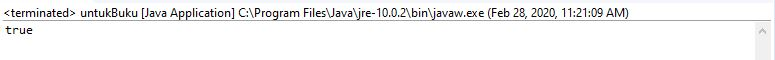
\includegraphics[scale=0.6]{pictures/operator_perbandingan_lebih_besar_sama_dengan.JPG}
                \caption{Hasil operator lebih besar sama dengan}
                \label{}
            \end{figure}

            \item \textbf{Lebih Kecil Sama Dengan}
            \begin{lstlisting}[language=Java]
public static void main(String[] args) {
    int A = 12;
    int B = 4;
    boolean hasil;
            
    // Apakah nilai A lebih kecil atau sama dengan nilai B?
    hasil = A <= B;
    System.out.println(hasil);
}
            \end{lstlisting}
            Hasil Eksekusi Program:
            \begin{figure}[htbp!]
                \centering
                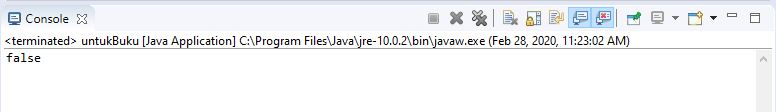
\includegraphics[scale=0.6]{pictures/operator_perbandingan_lebih_kecil_sama_dengan.JPG}
                \caption{Hasil operator lebih kecil sama dengan}
                \label{}
            \end{figure}

        \end{itemize}


    \item \textbf{Operator Bitwise}\\
    Operator bitwise fungsinya hampir sama dengan operator logika. Namun perbedaannya adalah operator bitwise digunakan untuk bilangan biner saja (bit). Operator bitwise terdir dari:
    \begin{table}[h!]
        \centering
        \begin{tabular}{|l|c|}
        \hline
        \rowcolor[HTML]{9AFF99} 
        \textbf{Nama}          & \multicolumn{1}{l|}{\cellcolor[HTML]{9AFF99}\textbf{Simbol}} \\ \hline
        AND                    & \&                                                           \\ \hline
        OR                     & |                                                            \\ \hline
        XOR                    & \textasciicircum{}                                           \\ \hline
        Negasi / Kebalikan     & $\sim$                                                       \\ \hline
        Left Shift             & \textless{}\textless{}                                       \\ \hline
        Right Shift            & \textgreater{}\textgreater{}                                 \\ \hline
        Left Shift (Unsigned)  & \textless{}\textless{}\textless{}                            \\ \hline
        Right Shift (Unsigned) & \textgreater{}\textgreater{}\textgreater{}                   \\ \hline
        \end{tabular}
        \caption{Operator Bitwise}
    \end{table}
    \newline
    Contoh penggunaan aplikasi bitwise:
    \begin{lstlisting}[language=Java]
        public static void main(String[] args) {
        int a = 60;    /* 60 = 0011 1100 */
        int b = 13;    /* 13 = 0000 1101 */
        int c = 0;

        c = a & b;       /* 12 = 0000 1100 */
        System.out.println("a & b = " + c);

        c = a | b;       /* 61 = 0011 1101 */
        System.out.println("a | b = " + c);

        c = a ^ b;       /* 49 = 0011 0001 */
        System.out.println("a ^ b = " + c);

        c = ~a;          /*-61 = 1100 0011 */
        System.out.println("~a = " + c);

        c = a << 2;     /* 240 = 1111 0000 */
        System.out.println("a << 2 = " + c);

        c = a >> 2;     /* 215 = 1111 */
        System.out.println("a >> 2  = " + c);

        c = a >>> 2;     /* 215 = 0000 1111 */
        System.out.println("a >>> 2 = " + c);
    }        
    \end{lstlisting}
    Hasil yang dikeluarkan adalah:
    \begin{figure}[htbp!]
        \centering
        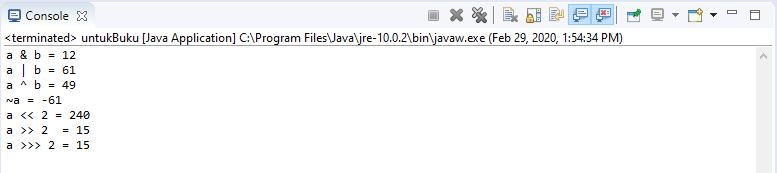
\includegraphics[scale=0.6]{pictures/operator_bitwise.JPG}
        \caption{Hasil Operator Bitwise}
        \label{}
    \end{figure}
\end{enumerate}

\section{Percabangan pada Java}
Percabangan merupakan pemilihan keputusan untuk mengeksekusi program berdasarkan kondisi yang ditetapkan. \cite{HengkyPercabangan}

Percabangan biasa disebut juga dengan \textit{Control Flow} yang merupakan perintah pada program agar program dapat mengambil keputusan. Percabangan akan menggunakan nilai \textbf{true} atau \textbf{false} dari beberapa kondisi yang terjadi.\\

Pada dasarnya dalam pemrograman terdapat 3 macam percabangan:
\begin{enumerate}
    \item Percabangan IF
    \item Percabangan IF/ELSE 
    \item Percabangan IF/ELSE/IF 
    \item Percabangan CASE
\end{enumerate}

\newpage
\subsection{Percabangan IF}
\begin{figure}[h!]
    \centering
    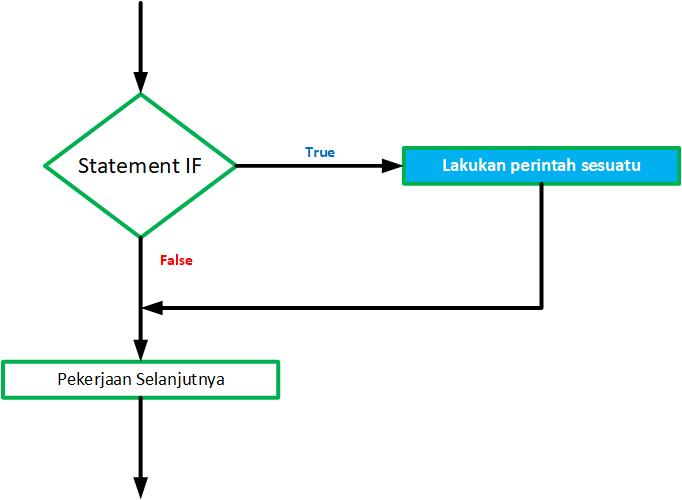
\includegraphics[scale=0.4]{pictures/flowmap_if.jpg}
    \caption{Alur logika percabangan IF}
    \label{}
\end{figure}
Percabangan IF hanya punya satu pilihan dan hanya akan dikerjakan kalau \textit{statementnya} bernilai benar. Jika \textit{statement} tidak bernilai benar, maka percabangan ini tidak bisa dijalankan. Bentuk dari IF adalah:
\begin{lstlisting}[language=Java]
if( statement ) {
    // perintah jika statement bernilai benar
    // perintah 1
    // perintah 2
    // dan seterusnya
}    
\end{lstlisting}

\textbf{Statement} hanya akan menghasilkan nilai \textbf{True} atau \textbf{False}. Untuk pengisian statement dapat digabungkan dengan operator logika, perbandingan, dan berbagai operator yang dapat digunakan dalam program. 

\medskip

\noindent\fcolorbox{red}{yellow}{%
    \minipage[b]{\dimexpr\linewidth\fboxsep\fboxrule\relax}
    Contoh dalam kegiatan sehari - hari adalah ketika kita belanja. Misalkan kita berbelanja diatas nominal 200.000 maka akan mendapat potongan harga.
    \endminipage}

\medskip

Jika contoh tersebut dibuat menjadi program maka akan menjadi:
\begin{lstlisting}[language=Java]
public static void main(String[] args) {

    // membuat variabel belanja dan scanner
    int belanja = 0;
    Scanner scan = new Scanner(System.in);

    // mengambil input
    System.out.print("Total Belanjaan: Rp ");
    belanja = scan.nextInt();

    // cek apakah dia belanja di atas 100000
    if ( belanja > 100000 ) {
        System.out.println("Selamat, anda mendapatkan hadiah!");
    }

    System.out.println("Terima kasih...");
}

\end{lstlisting}

\subsection{Percabangan IF/ELSE}
\begin{figure}[h!]
    \centering
    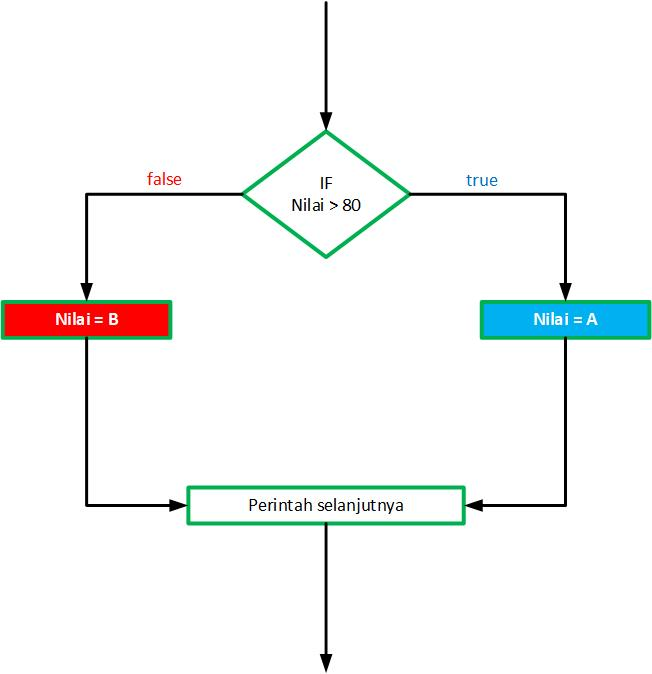
\includegraphics[scale=0.4]{pictures/flowmap_if_else.jpg}
    \caption{Alur logika percabangan if else}
    \label{}
\end{figure}

Percabangan IF/ELSE pada dasarnya hampir sama dengan percabangan IF diatas. Namun IF/ELSE memiliki perintah alternatif jika statement yang dijalankan bernilai false. 

Struktur dari IF/ELSE adalah:
\begin{lstlisting}[language=Java]
if (statement) {
    // perintah jika statement bernilai benar
    // perintah 1
    // perintah 2
    // dan seterusnya
} else {
    // perintah jika statement bernilai salah
    // perintah 1
    // perintah 2
    // dan seterusnya
}
\end{lstlisting}


\noindent\fcolorbox{red}{yellow}{%
    \minipage[b]{\dimexpr\linewidth\fboxsep\fboxrule\relax}
    Contoh dalam kegiatan sehari - hari adalah ketika dosen akan menentukan nilai hasil ujian akhir semester mahasiswa. Jika nilai mahasiswa > 80 maka nilai = A, dan jika nilai dibawah 80 maka nilai = B
    \endminipage}

\medskip

Bentuk Program dari contoh tersebut:
\begin{lstlisting}[language=Java]
public static void main(String[] args) {

    // membuat variabel Nilai dan scanner
    int nilai = 0;
    Scanner scan = new Scanner(System.in);

    // mengambil input
    System.out.print("Nilai: ");
    nilai = scan.nextInt();

    // cek apakah nilai UAS diatas 80?
    if (nilai > 80) {
        //jika hasil benar maka:
		System.out.println("Nilai: A");
	} else {
		//(Alternatif) Jika hasil salah maka: 
		System.out.println("Nilai: B");
	}

}   
\end{lstlisting}


Hasil dari program yang dijalankan adalah:
\begin{figure}[h!]
    \centering
    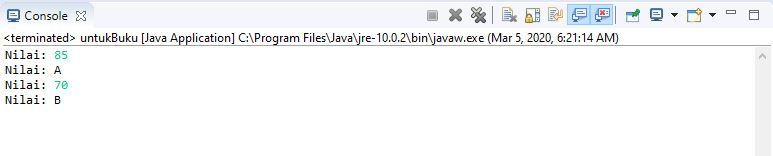
\includegraphics[scale=0.6]{pictures/hasil_if_else.jpg}
    \caption{Hasil program if else}
    \label{}
\end{figure}

\newpage
\subsection{Percabangan IF/ELSE/IF}
\begin{figure}[h!]
    \centering
    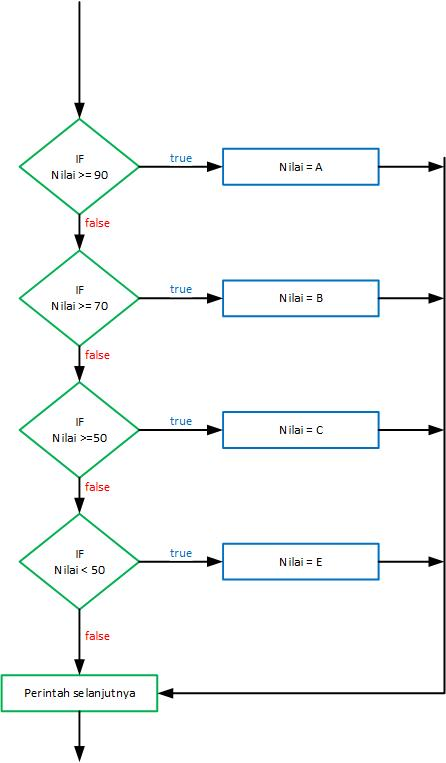
\includegraphics[scale=0.5]{pictures/flowmap_if_else_if.jpg}
    \caption{Flowmap logika IF/ELSE/IF}
    \label{}
\end{figure}

Jika kita lihat pada percabangan IF/ELSE hanya memiliki dua percabangan saja yaitu jika kondisi true dan false. Namun  pada percabangan IF/ELSE/IF, percabangan bisa memiliki banyak pilihan ketika kondisi yang dijalankan memiliki nilai false.

Struktur dari IF/ELSE/IF:
\begin{lstlisting}[language=Java]
if (statement 0) {
    // maka kerjakan perintah ini
    // perintah 1
    // perintah 2
    // ....
} else if (statement 1) {
    // kerjakan perintah ini
    // perintah 1
    // perintah 2
    // ....
} else if (statement 2) {
    // kerjakan perintah ini
    // perintah 1 juga
    // perintah 2 juga 
    // ....
} esle {
    // kerjakan perintah ini
    // hanya jika 
    // kondisi statement diatas tidak ada yang benar
    // ....
}    
\end{lstlisting}

\noindent\fcolorbox{red}{yellow}{%
    \minipage[b]{\dimexpr\linewidth\fboxsep\fboxrule\relax}
    Contoh dalam kegiatan sehari - hari adalah ketika dosen akan menentukan nilai grade dari mahasiswa. Jika Nilai >= 90 maka Grade = A, jika Nilai >= 70 maka Grade = B, jika Nilai >= 50 Grade C dan nilai < 50 maka Grade E.
    \endminipage}

\medskip

Bentuk contoh tersebut jika diubah menjadi bahasa program:
\begin{lstlisting}[language=Java]
public static void main(String[] args) {

    // membuat variabel Nilai dan scanner
    int nilai = 0;
    String grade;
        
    Scanner scan = new Scanner(System.in);

    // mengambil input
    System.out.print("Nilai: ");
        nilai = scan.nextInt();

    // IF/ELSE/IF untuk menentukan grade nilai mahasiswa 
    if ( nilai >= 90 ) {
        grade = "A";
    } else if ( nilai >= 70 ){
        grade = "B";
    } else if ( nilai >= 50 ){
        grade = "C";
    } else {
        grade = "E";
    }

    // Mencetak Grade dai nilai yang sudah diinputkan 
    System.out.println("Grade: " + grade);

}
\end{lstlisting}

Hasil dari program yang dijalankan adalah:
\begin{figure}[h!]
    \centering
    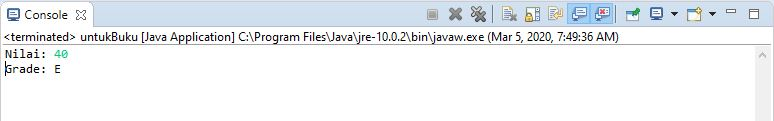
\includegraphics[scale=0.6]{pictures/hasil_if_else_if.JPG}
    \caption{Hasil program IF/ELSE/IF}
    \label{}
\end{figure}

\newpage
\subsection{Percabangan SWITCH/CASE}
\begin{figure}[h!]
    \centering
    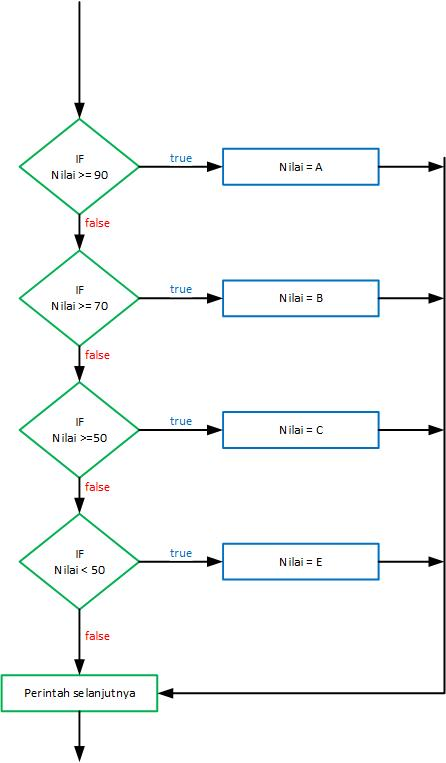
\includegraphics[scale=0.5]{pictures/flowmap_if_else_if.jpg}
    \caption{Flowmap logika SWITCH/CASE}
    \label{}
\end{figure}
Percabangan SWITCH/CASE secara fungsi hampir sama dengan percabangan IF/ELSE/IF namun pada percabangan ini perlu diingat bahwa kata kunci yang digunakan adalah \textcolor{pred}{switch} dan \textcolor{pred}{case}.

Bentuk program dari SWITCH/CASE adalah:
\begin{lstlisting}[language=Java]
switch(variabel){
    case 1:
        // Kerjakan perintah ini
        // perintah ini juga
        // perintah ini
        // ...
        break;
    case 2:
        // Kerjakan perintah ini
        // perintah ini juga
        // perintah ini
        // ...
        break;
    case 3:
        // Kerjakan perintah ini
        // perintah ini juga
        // perintah ini
        // ...
        break;
    default:
        // Kerjakan perintah ini
        // perintah ini juga
        // perintah ini
        // ...
	break;
}
\end{lstlisting}
Case 1 disini berisi Variabel yang akan dibandingkan sehingga memiliki hasil akhir true tau false.

\medskip

\noindent\fcolorbox{red}{yellow}{%
    \minipage[b]{\dimexpr\linewidth\fboxsep\fboxrule\relax}
    Contoh dalam kegiatan sehari - hari adalah ketika anda memiliki banyak pilihan seperti pada mesin ATM. Pada mesin ini disediakan beberapa pilihan menu seperti transfer, tarik tunai, cek saldo, dan lain-lain.
    \endminipage}

\medskip

Bentuk contoh tersebut jika diubah menjadi bahasa program:
\begin{lstlisting}[language = Java]
// membuat variabel dan Scanner
String pilihan;
Scanner scan = new Scanner(System.in);

// mengambil input
System.out.println("Selamat Datang di atm SNI");
System.out.println("1. Cek Saldo");
System.out.println("2. Tarik Tunai");
System.out.println("3. Setor");
System.out.println("Pilih Menu: ");
pilihan = scan.nextLine();

switch(pilihan){
    case "1":
        System.out.println("Saldo anda Rp.0,-");
        break;
    case "2":
        System.out.println("Anda Tidak Punya Saldo");
        break;
    case "3":
        System.out.println("Setor trosss");
        break;
    default:
        System.out.println("Masukan pilihan dengan benar!");
}
\end{lstlisting}

Hasil dari program yang dijalankan: 
\begin{figure}[h!]
    \centering
    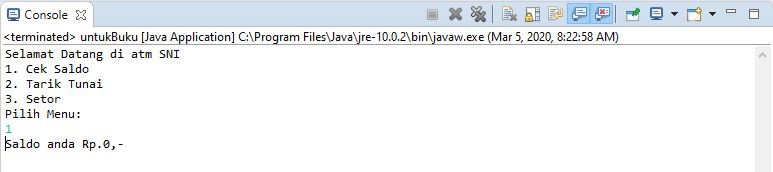
\includegraphics[scale=0.6]{pictures/hasil_switch_case.JPG}
    \caption{Hasil program SWITCH/CASE}
    \label{}
\end{figure}

\newpage
\subsection{Percabangan dalam percabangan (\textit{Nested})}
\begin{figure}[h!]
    \centering
    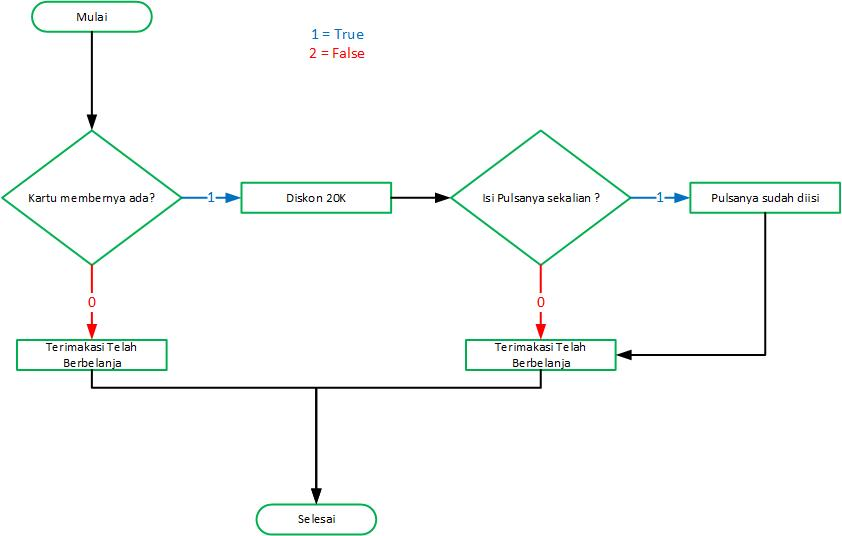
\includegraphics[scale=0.5]{pictures/flowmap_percabangan_dalam_percabangan.jpg}
    \caption{Flowmap logika percabangan dalam percabangan}
    \label{}
\end{figure}
Pada dasarnya percabangan dalam percabangan ini hampir sama dengan IF/ELSE karena menggunakanperintah \textcolor{pred}{if} dan \textcolor{pred}{else}. Namun ada if/else dalam if/else sehingga disebut "Percabangan dalam percabangan (\textit{Nested})"

Strukrur percabangan dalam percabangan:
\begin{lstlisting}[language=Java]
if (statement) {
        if (statement) {
            // Eksekusi perintah ini
            // Perintah ini
            // perintah itu
            // ....
        } else if (statement2) {
            // Eksekusi perintah ini
            // Perintah ini
            // perintah itu
            // ....
        } else {
            // Eksekusi perintah ini
            // Perintah ini
            // perintah itu
            // ....
        }

    } else {
        if (statement) {
            // Eksekusi perintah ini
            // Perintah ini
            // perintah itu
            // ....
        } else {
            // Eksekusi perintah ini
            // Perintah ini
            // perintah itu
            // ....
        }
    }
\end{lstlisting}

\medskip

\noindent\fcolorbox{red}{yellow}{%
    \minipage[b]{\dimexpr\linewidth\fboxsep\fboxrule\relax}
    Contoh dalam kegiatan sehari - hari adalah ketika membeli sesuatu di minimarket, kemudian kasir bertanya kartu member. Jika memiliki kartu member maka diskon 20.000 dan kasir akan bertanya lagi apakah akan isi pulsa sekalian? jika ya maka pulsa diisi, jika tidak maka selesai. Sedangkan jika tidak punya kartu member, Maka proses langsung selesai.
    \endminipage}

\medskip

Bentuk Contoh tersebut jika diubah menjadi bahasa program:
\begin{lstlisting}[language=Java]
// deklarasi variabel dan Scanner
String kartu, pulsa;
Scanner scan = new Scanner(System.in);

// mengambil input
System.out.print("Apakah ada kartu membernya?: ");
kartu = scan.nextLine();

// proses
if (kartu.equalsIgnoreCase("ya")) {
    System.out.println("Anda mendapat diskon 20.000");
    System.out.print("Mau isi pulsa sekalian?: ");
    pulsa = scan.nextLine();
    if (pulsa.equalsIgnoreCase("ya")) {
        System.out.println("Pulsa Terisi");
        System.out.println("Terimakasih telah berbelanja");
    } else if (pulsa.equalsIgnoreCase("tidak")) {
        System.out.println("Terimakasih telah berbelanja");
    } else {
        System.out.println("Terimakasih telah berbelanja");
    }

} else {
    System.out.println("Terimakasih telah berbelanja");
}
\end{lstlisting}

Hasil dari program yang dijalankan:
\begin{figure}[h!]
    \centering
    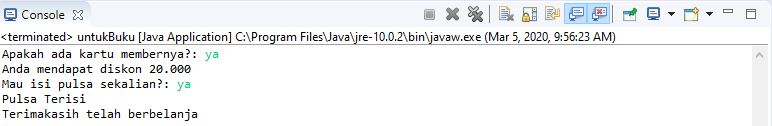
\includegraphics[scale=0.6]{pictures/hasil_percabangan_dalam_percabangan.JPG}
    \caption{Hasil program percabangan dalam percabangan}
    \label{}
\end{figure}








